\documentclass[12pt]{article}
\usepackage{geometry}
\usepackage{graphicx}
\usepackage{amsmath}
\usepackage{hyperref}
\usepackage{caption}
\usepackage{float}
% \usepackage{amsfonts}
% \usepackage{fontspec}
\usepackage{subcaption}
\usepackage{algorithm}
\usepackage{algpseudocode}


% \setmainfont{Latin Modern Roman} % or any installed font on your system

\geometry{a4paper, margin=1in}

\title{UrbanGraph: A Dynamic Urban Traffic Simulation Using Graph Algorithms}
\author{Ashkan Marali\\Alireza Sobhdoost}
\date{\today}

\begin{document}

\maketitle
\tableofcontents
\newpage

% ----------------------------------------
\section{Introduction}
UrbanGraph is a graph-based urban traffic simulation system designed to model and analyze user movements and traffic flow in a city-like environment. The system dynamically generates a random graph representing a city, where:
\begin{itemize}
    \item Nodes represent stations (in this case Universities).
    \item Edges represent roads connecting the nodes.
    \item The map is divided into four zones: North, South, East, and West—each with distinct colors.
\end{itemize}
Users (both automated and manual) traverse this graph, triggering algorithms like A* and TSP for route optimization and visualization.

% ----------------------------------------
\section{Clock and Tick System}
The system employs a discrete clock-based mechanism to simulate time-based events. Every 2 seconds (1 tick), two new random users are spawned on the graph. These users traverse the graph in a semi-random fashion to generate dynamic traffic patterns. This simulation enables a temporal evolution of congestion and allows for performance analysis of pathfinding algorithms under load.

\subsection{Tick Mechanics}
Each tick involves:
\begin{itemize}
    \item Spawning new users
    \item Assigning random start and destination nodes
    \item Updating the graph state and visual animation
\end{itemize}

\subsection{Traffic Management}

As users traverse the graph, traffic congestion is dynamically simulated and managed to reflect realistic movement limitations. Each edge in the graph has a defined \textbf{capacity}, representing the maximum number of simultaneous users it can support. When the number of users exceeds this threshold, the edge is considered \textit{congested}.

UrbanGraph handles congestion in two key ways:
\begin{itemize}
    \item \textbf{Routing Penalty:} A* pathfinding applies an additional cost when evaluating congested edges, making them less favorable for route selection.
    \item \textbf{Real-time Visualization:} Congested edges can be styled differently or animated with delay effects to reflect slowdown.
\end{itemize}


This mechanism ensures that traffic buildup influences user movement patterns over time, simulating a dynamic and reactive transport environment.

\vspace{1em}

\begin{figure}[H]
    \centering
    \begin{subfigure}[b]{0.48\textwidth}
        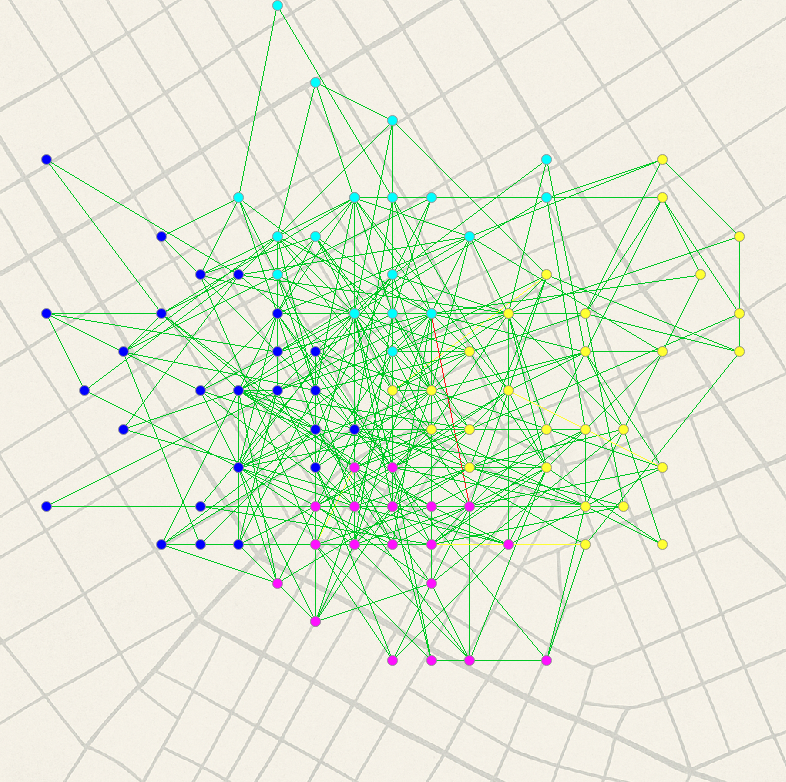
\includegraphics[width=\textwidth]{../Images/sample_img_1_2.png}
        \caption{100 node Graph under normal load conditions}
        \label{fig:traffic-normal}
    \end{subfigure}
    \hfill
    \begin{subfigure}[b]{0.48\textwidth}
        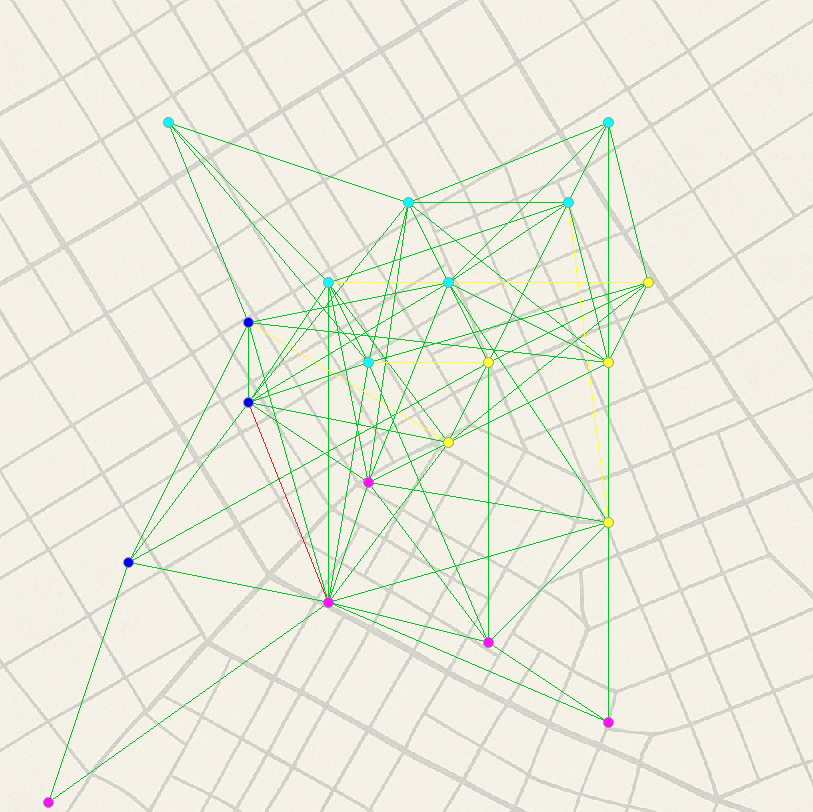
\includegraphics[width=\textwidth]{../Images/sample_img_2_1.png}
        \caption{20 node Graph under normal load conditions}
        \label{fig:traffic-congested}
    \end{subfigure}
    \caption{Comparison of traffic flow over time. As users accumulate, certain edges reach capacity limits and cause congestion-aware rerouting.}
    \label{fig:traffic-comparison}
\end{figure}


% ----------------------------------------
\section{Random Graph Generation}

The graph construction process in \textit{UrbanGraph} aims to simulate a realistic and fully connected urban layout. It begins by establishing a reliable connectivity structure using a \textbf{random spanning tree}, followed by the probabilistic addition of extra edges to introduce redundancy and improve path diversity.

\subsection{Spanning Tree Initialization}

To ensure the graph is initially connected, a random spanning tree is generated. The process begins by selecting a random node as the starting point. Then, nodes are incrementally connected in a randomized fashion: each new edge links a randomly chosen \textit{visited} node to a randomly chosen \textit{unvisited} node. This continues until all nodes are connected. The resulting edge set forms a spanning tree — a minimal structure with no cycles that connects all nodes.

\subsection{Edge Densification}

While a spanning tree ensures connectivity, it offers only a single unique path between any two nodes, which is not reflective of real-world road networks. To address this, the algorithm adds a number of extra edges (approximately 2.5 times the number of nodes) to increase path redundancy. These edges are selected using a distance-weighted probabilistic approach:
\begin{itemize}
    \item Candidate node pairs are selected at random.
    \item The probability of adding an edge between them decreases exponentially with their Euclidean distance.
\end{itemize}
This technique favors local connections, encouraging dense clusters and realistic neighborhood patterns, while occasionally allowing longer edges that connect distant zones, simulating arterial roads.

\subsection{Node Positioning and Layout}

Once the edge set is finalized, a spring layout algorithm is used to assign spatial coordinates to the nodes. This layout algorithm models edges as springs and places nodes in two-dimensional space in a way that minimizes edge crossing and distributes nodes uniformly.

To standardize rendering, the final layout is centered around the origin and scaled, with coordinates rounded to simplify zone computation and rendering precision.

\subsubsection*{Node Interaction View}

UrbanGraph also supports an interactive view where clicking on a node reveals only its directly connected edges. This feature helps users inspect local connectivity and understand how each node integrates into the larger graph.

\begin{figure}[H]
    \centering
    \begin{subfigure}[b]{0.48\textwidth}
        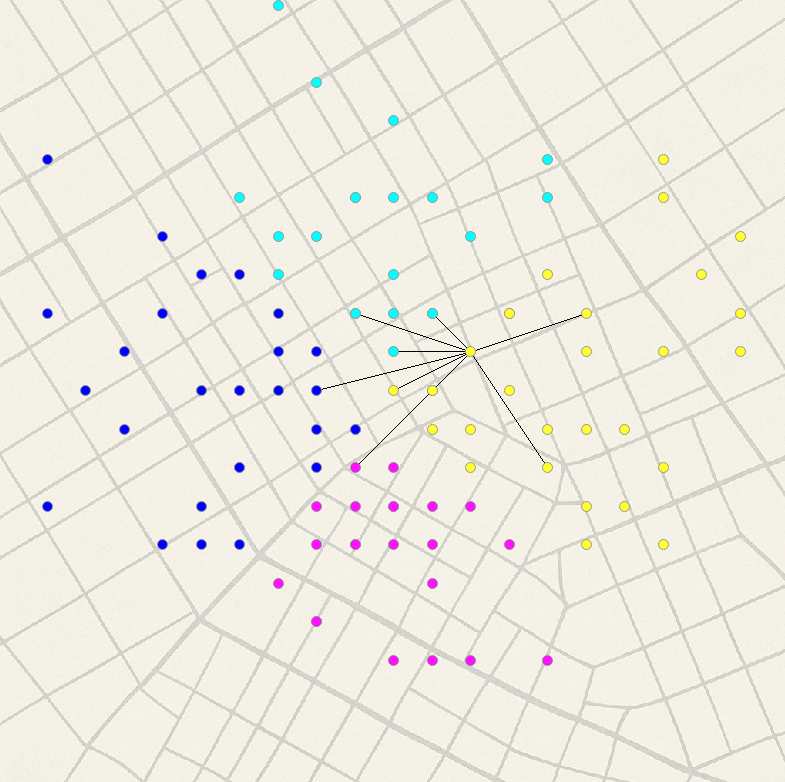
\includegraphics[width=\textwidth]{../Images/sample_img_1_1.png}
        \label{fig:node-click-1}
    \end{subfigure}
    \hfill
    \begin{subfigure}[b]{0.48\textwidth}
        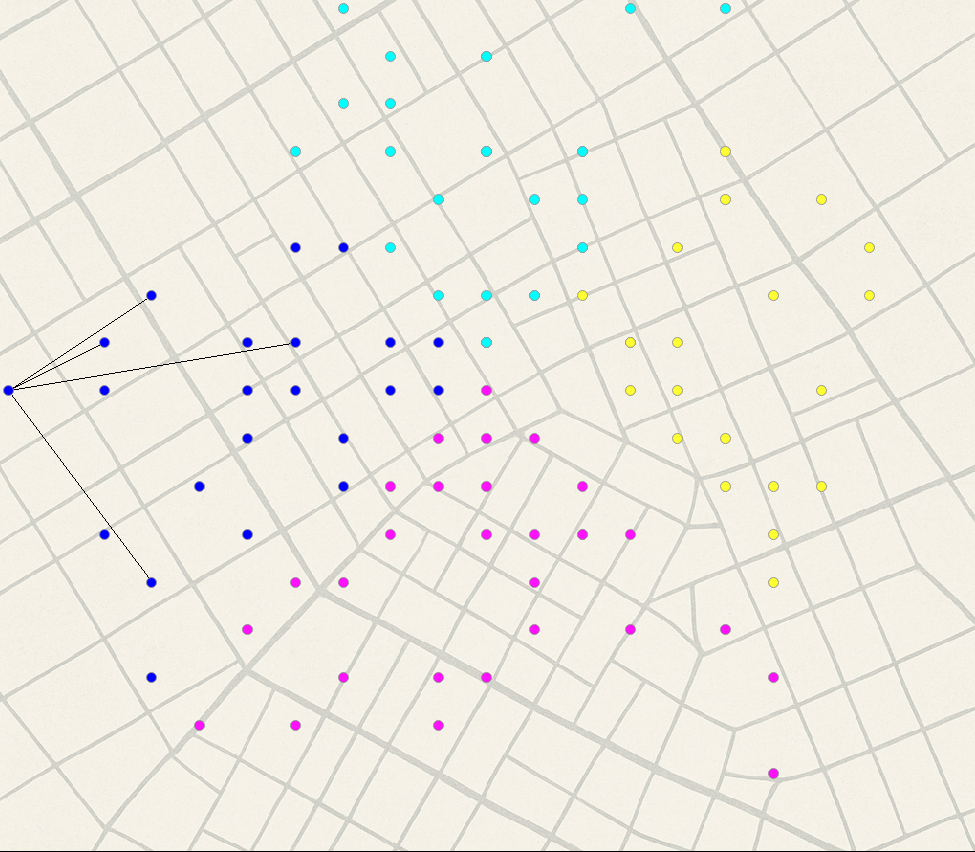
\includegraphics[width=\textwidth]{../Images/sample_img_3_1.png}
        \label{fig:node-click-2}
    \end{subfigure}
    \caption{Interactive node selection views. Only edges connected to the selected node are shown, enhancing clarity of local structure.}
    \label{fig:node-click-pair}
\end{figure}


\subsection{Zone Assignment}

Each node in the graph is assigned to one of four spatial zones based on its $(x, y)$ coordinates. The assignment prioritizes vertical separation (North/South) over horizontal (East/West), ensuring a consistent and intuitive layout.

\begin{itemize}
    \item \textbf{North (Zone 0)}: $|y| > |x|$ and $y \geq 0$ \\
          \textit{Color: Cyan (\texttt{\#17becf})}
    \item \textbf{South (Zone 1)}: $|y| > |x|$ and $y < 0$ \\
          \textit{Color: Magenta (\texttt{\#e377c2})}
    \item \textbf{East (Zone 2)}: $|x| \geq |y|$ and $x \geq 0$ \\
          \textit{Color: Yellow (\texttt{\#bcbd22})}
    \item \textbf{West (Zone 3)}: $|x| \geq |y|$ and $x < 0$ \\
          \textit{Color: Blue (\texttt{\#1f77b4})}
\end{itemize}
% ----------------------------------------
\begin{figure}[H]
    \centering
    \begin{subfigure}[b]{0.48\textwidth}
        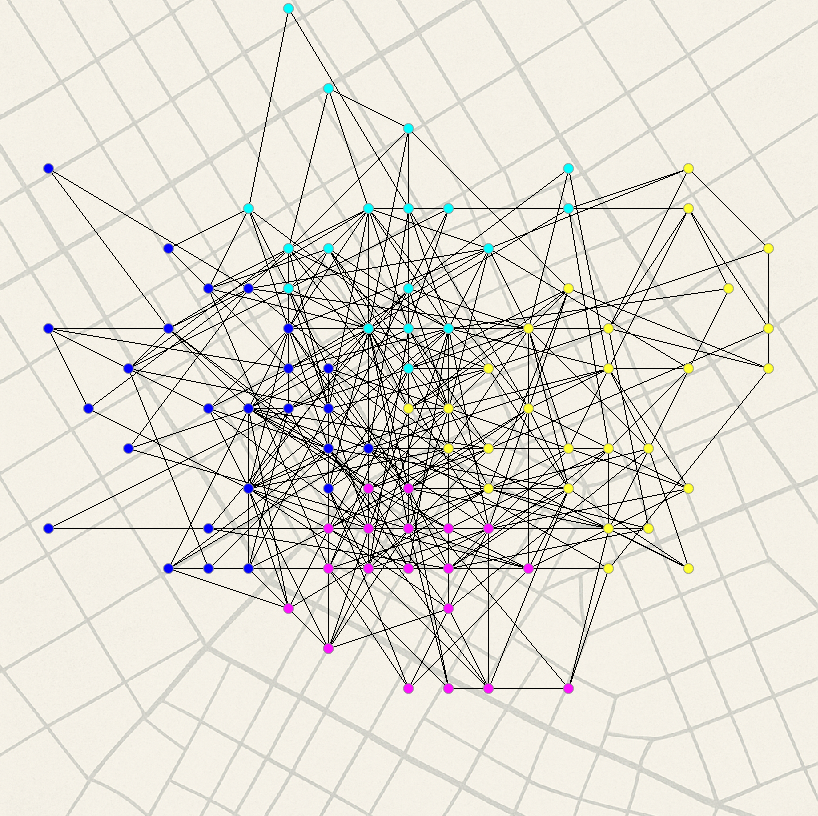
\includegraphics[width=\textwidth]{../Images/sampleMap_1.png}
        \caption{100 node Graph}
        \label{fig:mst-1}
    \end{subfigure}
    \hfill
    \begin{subfigure}[b]{0.48\textwidth}
        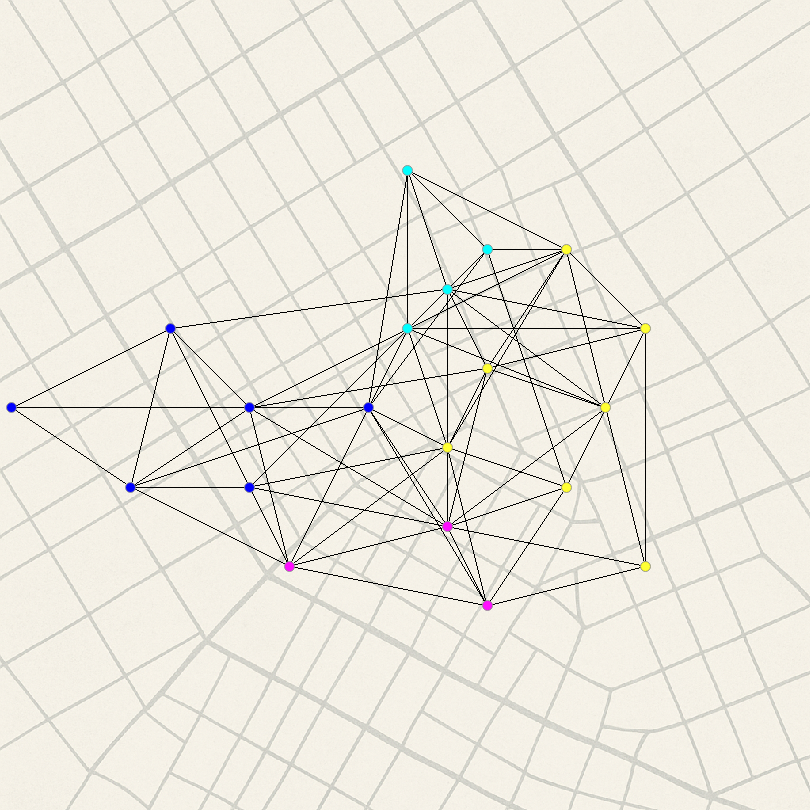
\includegraphics[width=\textwidth]{../Images/sampleMap_2.png}
        \caption{20 node Graph}
        \label{fig:mst-2}
    \end{subfigure}
    \caption{Visualizations of the UrbanGraph map with nodes colored by zone. Each zone is represented by a distinct color, enhancing spatial understanding of the graph structure.}
    \label{fig:mst-both}
\end{figure}

% \newpage

\section{Travel and Route Computation}
\subsection{A* Pathfinding Algorithm}

UrbanGraph uses the A* search algorithm to compute efficient travel routes between stations (nodes) within the city graph. A* is chosen for its balance of performance and optimality, combining the benefits of Dijkstra's algorithm with heuristic-driven search.

\subsubsection*{Heuristic Design}

The heuristic used in UrbanGraph considers two factors:
\begin{itemize}
    \item \textbf{Geometric Distance}: The Euclidean distance between the current node and the goal node.
    \item \textbf{Zone Transition Cost}: A penalty based on the number of zone boundaries crossed (e.g., moving from South to East). This is weighted to encourage intra-zone travel when possible.
\end{itemize}

The final heuristic formula is:
\[
h(n) = 0.7 \cdot \text{distance}(n, \text{goal}) + 0.3 \cdot \text{zone\_difference}(n, \text{goal}) \times 10
\]
This allows the algorithm to prioritize spatial proximity while still accounting for logical travel costs between urban zones.

\subsubsection*{Edge Handling and Traffic Sensitivity}

Each edge has a defined capacity. If an edge is congested (i.e., its number of current passengers exceeds capacity), a penalty is applied to its weight to simulate traffic delays. This discourages the algorithm from routing through heavily congested areas unless no better options exist. Congestion is handled as follows:
\begin{itemize}
    \item Normal edge: uses base weight.
    \item Congested edge: weight is increased by a penalty factor.
\end{itemize}

\subsubsection*{Multi-Zone Travel and Border Nodes}

When a route spans multiple zones (e.g., from North to West), UrbanGraph uses a two-phase strategy involving \textbf{border nodes}, which are nodes located near zone boundaries and flagged during graph preprocessing:
\begin{enumerate}
    \item Compute paths from the start node to all possible border nodes in the target zone.
    \item For each such border, compute a secondary path to the final goal.
    \item Select the combination with the lowest total cost.
\end{enumerate}

\begin{algorithm}
    \caption{A* Search with Zone Handling}
    \label{alg:a_star_zone}
    \begin{algorithmic}[1]
    \Procedure{PerformAStar}{$start\_node$, $goal\_node$, $border\_nodes$}
        \State $node1\_zone \gets start\_node.zone$
        \State $node2\_zone \gets goal\_node.zone$
        
        \If{$node1\_zone == node2\_zone$}
            \State \Return \Call{AStarSearch}{$start\_node$, $goal\_node$}
        \EndIf
        
        \State $key \gets \text{concat}(\min(node1\_zone, node2\_zone), \text{"to"}, \max(node1\_zone, node2\_zone))$
        \State $best\_cost \gets \infty$
        \State $best\_path \gets \text{None}$
        \State $best\_edges \gets \text{None}$
        
        \If{$border\_nodes.\text{get}(key)$}
            \State $candidates \gets border\_nodes[key]$
        \Else
            \State $trimed\_dict \gets$ \Call{FilterBorderByZone}{$node1\_zone$, $border\_nodes$}
            \State $candidates \gets$ \text{list of nodes from} $trimed\_dict$ \text{where nodes exist}
        \EndIf
        
        \For{$border\_node$ \textbf{in} $candidates$}
            \State $(path1, edges1) \gets$ \Call{AStarSearch}{$start\_node$, $border\_node$}
            \State $(path2, edges2) \gets$ \Call{AStarSearch}{$border\_node$, $goal\_node$}
            
            \If{$path1 == \text{None}$ \textbf{or} $path2 == \text{None}$}
                \State \textbf{continue}
            \EndIf
            
            \State $cost \gets \sum(e.weight$ \textbf{for} $e$ \textbf{in} $edges1 + edges2)$
            
            \If{$cost < best\_cost$}
                \State $best\_cost \gets cost$
                \State $best\_path \gets path1[:-1] + path2$
                \State $best\_edges \gets edges1 + edges2$
            \EndIf
        \EndFor
        
        \State \Return $(best\_path, best\_edges)$
    \EndProcedure
    \end{algorithmic}
    \end{algorithm}

This design reduces unnecessary zone-hopping and makes routing more efficient and realistic in zoned urban networks. You can see our recursive D\&Q algorithm in algorithm\ref{alg:a_star_zone}

\subsubsection*{Output}

The A* algorithm returns:
\begin{itemize}
    \item A list of nodes representing the optimal path.
    \item A corresponding list of edges traversed, used for animation and visualization.
\end{itemize}

If no valid path is found (e.g., all routes are blocked or unreachable), the algorithm returns a failure state, which is handled by the interface.

\subsubsection*{Visualization}

The selected path is animated on the graph, with directional highlighting of edges. Congested paths can be visually distinguished by their traversal delay or special styling.

\subsection{Traveling Salesman Problem (TSP) with A*}

In addition to computing shortest paths between two individual points, UrbanGraph supports multi-goal pathfinding by integrating the \textbf{Traveling Salesman Problem (TSP)}. This allows a user to select multiple destinations, and the system computes the most efficient route that visits all of them starting from a source node.

\subsubsection*{Approach}

The solution uses a dynamic programming (DP) approach to approximate the optimal path while incorporating real route costs obtained from the A* algorithm. This hybrid method is both computationally efficient and spatially realistic in an urban navigation context.

\subsubsection*{Graph-Aware Cost Matrix}

A key part of this implementation is the construction of a distance matrix between the source node and all destination nodes:
\begin{itemize}
    \item A* is used to compute the actual travel cost from the source to each destination.
    \item A pairwise cost is computed between every two destination nodes using A* again.
    \item The resulting matrix reflects real traversal costs that consider traffic, edge weights, and zone transitions.
\end{itemize}

\subsubsection*{Dynamic Programming Formulation}

The algorithm constructs a DP table where:
\begin{itemize}
    \item Each state represents a bitmask of visited nodes.
    \item Each entry tracks the minimum cost to reach a subset of destinations ending at a particular node.
    \item Transitions update the table by considering the cost of moving from one node to another, using the precomputed A* distances.
\end{itemize}

The goal is to find the minimum-cost path that visits all destinations exactly once.

The TSP solution constructs a dynamic programming (DP) matrix to track the minimum cost of reaching each subset of destinations. The matrix is defined as:

\[
\text{dp}[S][j] = \text{minimum cost to reach destination } j \text{ having visited the set } S
\]

where:
\begin{itemize}
    \item \( S \) is a bitmask representing a subset of visited destinations.
    \item \( j \in [0, n-1] \) is the index of the last visited destination.
    \item \( n \) is the total number of destinations.
    \item Costs are computed using A* for each path between destination nodes.
\end{itemize}

\vspace{1em}

An example for \( n = 3 \) destinations (\( D_0, D_1, D_2 \)):

\[
\begin{array}{c|ccc}
\textbf{Mask (S)} & D_0 & D_1 & D_2 \\
\hline
000 & \infty & \infty & \infty \\
001 & c_{s \rightarrow D_0} & \infty & \infty \\
010 & \infty & c_{s \rightarrow D_1} & \infty \\
100 & \infty & \infty & c_{s \rightarrow D_2} \\
011 & c_{D_1 \rightarrow D_0} & c_{D_0 \rightarrow D_1} & \infty \\
101 & c_{D_2 \rightarrow D_0} & \infty & c_{D_0 \rightarrow D_2} \\
110 & \infty & c_{D_2 \rightarrow D_1} & c_{D_1 \rightarrow D_2} \\
111 & \cdots & \cdots & \cdots \\
\end{array}
\]

Here:
\begin{itemize}
    \item Each row corresponds to a bitmask subset of visited destinations.
    \item Each column represents the destination node the path ends at.
    \item \( c_{u \rightarrow v} \) denotes the A*-computed cost from node \( u \) to node \( v \).
    \item Initial entries are seeded using costs from the source node.
\end{itemize}

The final result is taken from the row corresponding to \( S = 111 \) (all destinations visited), and the column with the lowest value.


\subsubsection*{Path Reconstruction}

Once the DP table is filled:
\begin{enumerate}
    \item The end node with the lowest cost is selected.
    \item The path is backtracked through the DP table to recover the node visitation sequence.
    \item A* is rerun on each segment to regenerate the exact node and edge path for animation and visualization.
\end{enumerate}

\subsubsection*{Features and Benefits}


\begin{itemize}
    \item Realistic cost modeling through A* integration.
    \item Considers zone boundaries and traffic conditions.
    \item Efficient even for moderate numbers of destinations (up to 10–15).
    \item Produces paths ready for smooth animation in the user interface.
\end{itemize}

\subsubsection*{Output}

The algorithm outputs:
\begin{itemize}
    \item Total estimated travel cost
    \item The optimal node visitation sequence
    \item A list of nodes and edges traversed (with duplicate suppression)
\end{itemize}

This system enhances UrbanGraph’s utility in logistics and route planning scenarios where multiple stops must be handled optimally.


% ----------------------------------------
\section{Minimum Spanning Tree (MST)}

UrbanGraph includes an interactive visualization of the \textbf{Minimum Spanning Tree (MST)} of the graph, computed using Prim’s algorithm. This allows users to explore the minimal structure that connects all stations (nodes) with the least total edge cost.

\subsection*{Prim's Algorithm Overview}

The MST is generated using a variant of Prim’s algorithm:
\begin{itemize}
    \item The algorithm begins at an arbitrary start node.
    \item At each step, it adds the minimum-weight edge that connects a visited node to an unvisited one.
    \item This continues until all nodes have been included in the MST.
\end{itemize}

Each edge in the MST retains metadata such as weight, capacity, and color, ensuring consistency with the original graph and enabling intuitive visualization.

\subsection*{MST Construction and Properties}

The algorithm operates on an adjacency list representation of the graph. Edges are prioritized by weight using a min-heap structure. Additional properties preserved in the MST include:
\begin{itemize}
    \item \textbf{Edge Capacity}: Used for potential traffic simulation.
    \item \textbf{Color}: Each MST edge inherits its color from the original edge for zone consistency.
\end{itemize}

The total weight of the MST is calculated and can be used to assess the minimal infrastructure cost of keeping the network connected.


\subsection*{Interactive Visualization}

UrbanGraph generates a separate, interactive plot of the MST that includes:
\begin{itemize}
    \item \textbf{Nodes}: Colored according to their zone.
    \item \textbf{MST Edges}: Drawn using the original edge color and rendered with increased thickness.
    \item \textbf{Labels}: Node IDs are overlaid for identification and analysis.
\end{itemize}

\begin{figure}[H]
    \centering
    \begin{subfigure}[b]{0.48\textwidth}
        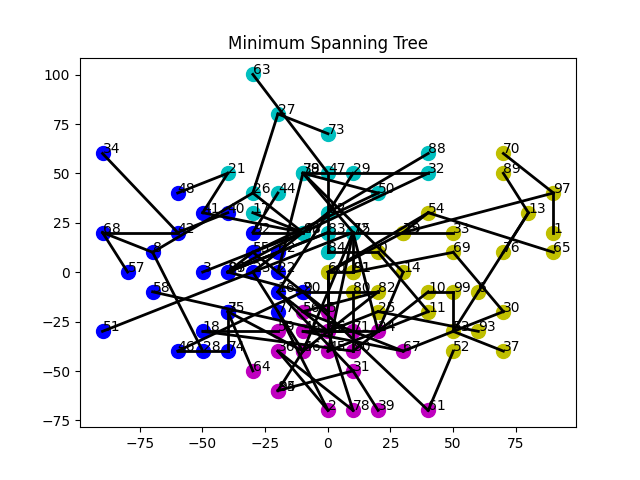
\includegraphics[width=\textwidth]{../Images/sampleMST_1.png}
        \caption{MST for a 100 node Graph}
        \label{fig:mst-1}
    \end{subfigure}
    \hfill
    \begin{subfigure}[b]{0.48\textwidth}
        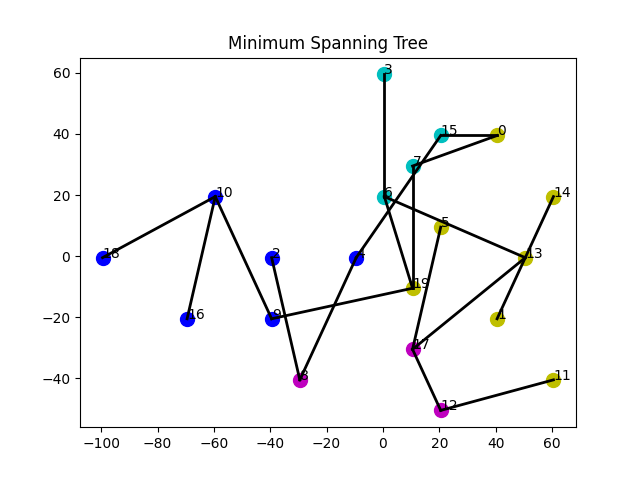
\includegraphics[width=\textwidth]{../Images/sampleMST_2.png}
        \caption{MST for a 20 node Graph}
        \label{fig:mst-2}
    \end{subfigure}
    \caption{Visualizations of the Minimum Spanning Tree (MST) in UrbanGraph. Edges reflect minimal-cost connections and node zones.}
    \label{fig:mst-both}
\end{figure}


This visualization enables users to explore the MST structure independently of the full traffic simulation and can serve educational, analytical, or debugging purposes.

\subsection*{Applications}

The MST mode serves multiple roles within UrbanGraph:
\begin{itemize}
    \item Visualizing the core backbone of the network.
    \item Comparing full connectivity versus minimal connection models.
    \item Supporting future integration with cost-optimized planning tools.
\end{itemize}

The MST module thus enhances UrbanGraph’s ability to serve as both a dynamic simulation and a structural analysis platform.

% ----------------------------------------
\section{Breadth-First Search (BFS)}

UrbanGraph includes support for performing and visualizing \textbf{Breadth-First Search (BFS)} from any node selected by the user. BFS provides a level-wise exploration of the network and is a valuable tool for educational purposes and spatial analysis.

\subsection*{Traversal Mechanism}

Breadth-First Search is initiated from a user-selected node and proceeds by exploring all neighboring nodes before moving outward to the next level. It uses a queue to maintain traversal order and a set to track visited nodes, ensuring each node is visited only once.

\begin{itemize}
    \item The algorithm begins at the selected start node.
    \item It explores all directly connected neighbors.
    \item This process continues layer by layer until all reachable nodes are visited.
\end{itemize}

The final path represents the order in which nodes were discovered.

\subsection*{Interactive Visualization}

UrbanGraph renders the BFS traversal in an interactive and visual format:
\begin{itemize}
    \item \textbf{Nodes}: Displayed and colored according to their zone.
    \item \textbf{Original Edges}: Shown in the background with partial transparency.
    \item \textbf{Traversal Path}: The path of visited nodes is overlaid with a dashed blue line.
    \item \textbf{Start Node}: Highlighted in green with a black border.
    \item \textbf{Final Node}: Highlighted in red with a black border.
\end{itemize}

\begin{figure}[H]
    \centering
    \begin{subfigure}[b]{0.48\textwidth}
        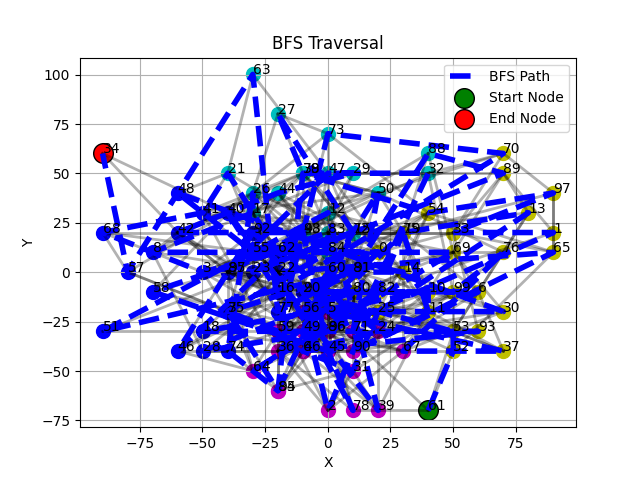
\includegraphics[width=\textwidth]{../Images/sampleBFS_1.png}
        \caption{BFS for a 100 node Graph}
        \label{fig:bfs-1}
    \end{subfigure}
    \hfill
    \begin{subfigure}[b]{0.48\textwidth}
        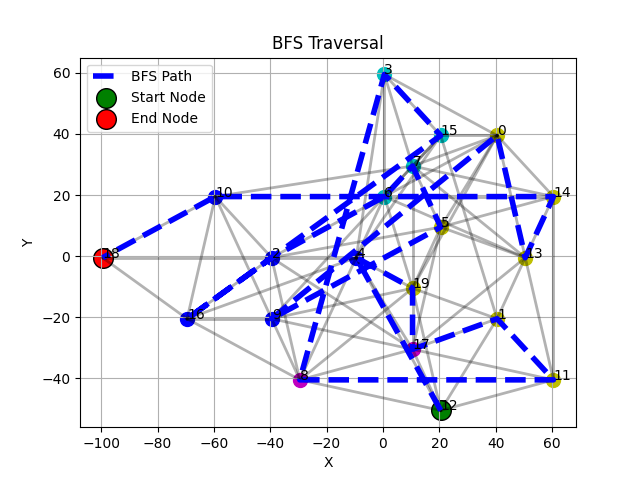
\includegraphics[width=\textwidth]{../Images/sampleBFS_2.png}
        \caption{BFS for a 100 node Graph}
        \label{fig:bfs-2}
    \end{subfigure}
    \caption{Visualizations of Breadth-First Search (BFS) traversal in UrbanGraph. The dashed blue line shows traversal order, with start and end nodes clearly highlighted.}
    \label{fig:bfs-both}
\end{figure}


This layout allows users to visually trace the breadth-first exploration in both spatial and logical order.

\subsection*{Use Cases}

The BFS module serves several practical and pedagogical roles:
\begin{itemize}
    \item Understanding the structure and density of local neighborhoods.
    \item Visualizing how search algorithms propagate in a graph.
    \item Validating graph connectivity in real time.
\end{itemize}

\subsection*{Integration with Simulation}

Though BFS is not used for routing in UrbanGraph, it provides insight into the graph's topology and complements other algorithmic features such as A* and MST. Users may invoke BFS at any time during the simulation for exploration or analysis.


% ----------------------------------------
\section{Time and Space Complexity}

This section analyzes the time and space complexity of the major algorithms used in \textit{UrbanGraph}. Each algorithm is evaluated in terms of its computational efficiency with respect to the number of nodes \( n \) and edges \( e \) in the graph.

\subsection*{A* Search}

A* combines Dijkstra’s algorithm with a heuristic function to prioritize exploration.

\begin{itemize}
    \item \textbf{Time Complexity:} \( O(e \log n) \) when using a binary heap for the priority queue. In dense graphs or with many neighbors, the runtime can approach \( O(n^2) \).
    \item \textbf{Space Complexity:} \( O(n) \) for storing scores, visited nodes, and the open/closed sets.
\end{itemize}

The heuristic function used in UrbanGraph includes both geometric distance and zone transition penalties, improving performance in spatially structured networks.

\subsection*{TSP Solver (with A* Cost Evaluation)}

The TSP module employs a dynamic programming solution with bitmasking to track subsets of visited destinations, and A* is used to compute real pairwise distances.

\begin{itemize}
    \item \textbf{Time Complexity:} \( O(n^2 \cdot 2^n) \), where \( n \) is the number of destinations.
    \item \textbf{Space Complexity:} \( O(n \cdot 2^n) \) for storing the DP table.
\end{itemize}


\subsection*{Minimum Spanning Tree (MST)}

UrbanGraph computes the MST using Prim’s algorithm with a priority queue.

\begin{itemize}
    \item \textbf{Time Complexity:} \( O(e \log n) \) when using a binary heap.
    \item \textbf{Space Complexity:} \( O(n + e) \) for storing the graph structure and MST.
\end{itemize}

This algorithm ensures full connectivity with minimal total weight and supports filtering by zone.

\subsection*{Breadth-First Search (BFS)}

BFS is used for level-order exploration of the graph starting from a selected node.

\begin{itemize}
    \item \textbf{Time Complexity:} \( O(n + e) \) — each node and edge is visited once.
    \item \textbf{Space Complexity:} \( O(n) \) for the visited set and queue.
\end{itemize}

% ----------------------------------------
\section{Conclusion}
UrbanGraph offers a modular and visually engaging way to explore pathfinding and graph algorithms in an urban context. The simulation demonstrates how computational strategies can be applied to traffic and logistics challenges.

% ----------------------------------------
\end{document}